\chapter{Theoretical background}
\label{DFT-chapter}
In this chapter, an overview of the theory behind the calculations performed throughout the attached manuscripts is available. It introduces the Density Functional Theory (DFT) as well as snippets description on the used functionals and their development.
\section{The many-body problem}
The solution of any quantum mechanical problem is obtained by evaluating the eigenvalues and eigenfunctions of the Hamiltonian operator ($H\Psi=E\Psi$) formulated in equation \ref{manybodyH}. Since the exact solution of such equation for a many-body system is analytically impossible, therefore a series of approximations are to be applied. In this chapter, we briefly discuss basic theories and approximations, which formulates the density functional theory. The many-body Hamiltonian is formulated as in equation \ref{manybodyH}:
\begin{multline}
\hat{H}=\,\,\,\,-\,\,\,\,\overbrace{\frac{\hbar^2}{2}\sum_{I}{\frac{\nabla_I^2}{M_I}}}^\textrm{Nuclei K.E.}\,\,\,\,+\,\,\,\,\overbrace{{1 \over 2} \sum_{I \neq J}{\frac{Z_I Z_J e^2}{4\pi\epsilon_0\abs{\vec{R_I}-\vec{R_J}}}}}^\textrm{Nucleus-Nucleus Interaction}\,\,\,\,-\,\,\,\,\overbrace{\frac{\hbar^2}{2m}\sum_{i}{\nabla_i^2}}^\textrm{Electrons K.E.}\\ \,\,\,\,+\,\,\,\,\underbrace{{1 \over 2} \sum_{i \neq j}{\frac{e^2}{4\pi\epsilon_0\abs{\vec{r_i}-\vec{r_j}}}}}_\textrm{Electron-Electron Interaction}\,\,\,\,-\,\,\,\,\underbrace{ \sum_{i,  I}{\frac{Z_I {e^2}}{4\pi\epsilon_0\abs{\vec{r_i}-\vec{R_I}}}}}_\textrm{\, \, Electron-Nucleus Interaction}
\label{manybodyH}
\end{multline}

In the many-body Hamiltonian: the first term $\left[-\frac{\hbar^2}{2}\sum_{I}{\frac{\nabla_I^2}{M_I}} \right]$ represents the kinetic energy of all nuclei, each with mass $M_I$. The second term $\left[ {1 \over 2} \sum_{I \neq J}{\frac{Z_I Z_Je^2}{4\pi\epsilon_0\abs{\vec{R_I}-\vec{R_J}}}}\right]$ represents nucleus-nucleus interactions via Coulomb repulsive forces. The second term can be calculated efficiently using Ewald's summation method (which determines the electrostatic potential as well as the energy of point charges in a crystal~\cite{Prasanna2012}). The third term $\left[ -\frac{\hbar^2}{2m}\sum_{i}{\nabla_i^2} \right]$ represents the kinetic energy of electrons, each with mass $m$. The fourth term $\left[ {1 \over 2} \sum_{i \neq j}{\frac{e^2}{4\pi\epsilon_0\abs{\vec{r_i}-\vec{r_j}}}} \right]$ represents the Coulomb interaction within pairs of electrons (the so called Hartree interaction). The fifth and last term $\left[-\sum_{i,I}{\frac{Z_I e^2}{4\pi\epsilon_0\abs{\vec{r_i}-\vec{R_I}}}} \right]$ represents electron-nucleus Coulomb interactions. The $1/2$ in the electron-electron and nucleus-nucleus interactions is to correct for the double counting.
% when we do the sum over i not equal j
% we are counting 1 with 2 and 2 with 1
% so the same term we counted twice
% because it is the same interaction, so, we put 1/2

The first step to simplify the many-body Hamiltonian is to invoke the Born-Oppenheimer approximation, detailed in the following section.
\section{Born-Oppenheimer approximation}
\label{BO}
% Since the nucleus is at least two thousand times heavier than the electron, the motion of a nucleus is much slower than that of an electron. Therefore the first approximation to introduce here, is taking the kinetic energy of nuclei to be zero in equation~(\ref{manybodyH}). \\
The Born-Oppenheimer approximation~\cite{Born1998} (BO) simplifies the solution of the many-body Schr\"{o}dinger equation (equation~\ref{manybodyH}) as it separates the nuclear and electronic motion. This approximation leads to two wave equations. The first equation describes the electronic motion, which can be solved separately by further approximations to evaluate the electronic wave function and the ground state energy. The second equation provides a description of the motion of the nuclei.\footnote{The contents of this section and the upcoming sections closely follows the presentation in standard textbooks in the subject, e.g., ABC of DFT~\cite{ABCofDFT} and Density Functional Theory and the family of (L)APW-methods: a step-by-step introduction~\cite{planewaveBook}.} The final result is the simplified Born-Oppenheimer Hamiltonian described in equation~\ref{BOHamiltonian} below:
\begin{multline}
\hat{H}^{\text{BO}}=\,\,\,\,-\,\,\,\,\underbrace{\frac{\hbar^2}{2m}\sum_{i}{\nabla_i^2}}_\textrm{Electrons K.E.}\,\,\,\,+\,\,\,\,\underbrace{{1 \over 2} \sum_{i \neq j}{\frac{e^2}{4\pi\epsilon_0\abs{\vec{r_i}-\vec{r_j}}}}}_\textrm{Electron-Electron Interaction}\\
\,\,\,\,-\,\,\,\,\underbrace{\sum_{i,I}{\frac{Z_Ie^2}{4\pi\epsilon_0\abs{\vec{r_i}-\vec{R_I}}}}}_\textrm{Electron-Nucleus Interaction}\,\,\,\,+\,\,\,\,\underbrace{{1 \over 2} \sum_{I \neq J}{\frac{Z_I Z_Je^2}{4\pi\epsilon_0\abs{\vec{R_I}-\vec{R_J}}}}}_\textrm{Nucleus-Nucleus Interaction}
\label{BOHamiltonian}
\end{multline}

In atomic units, the Born-Oppenheimer Hamiltonian is expressed in equation~\ref{BOHamiltonianAtomic} with $\hbar=m_e=e=4\pi\epsilon_0=1$ as: 
\begin{multline}
\hat{H}^{\text{BO}}=\,\,\,\,-\,\,\,\,\underbrace{\frac{1}{2}\sum_{i}{\nabla_i^2}}_\textrm{Electrons K.E.}\,\,\,\,+\,\,\,\,\underbrace{{1 \over 2} \sum_{i \neq j}{\frac{1}{\abs{\vec{r_i}-\vec{r_j}}}}}_\textrm{Electron-Electron Interaction}\\
\,\,\,\,-\,\,\,\,\underbrace{\sum_{i,I}{\frac{Z_I}{\abs{\vec{r_i}-\vec{R_I}}}}}_\textrm{Electron-Nucleus Interaction}\,\,\,\,+\,\,\,\,\underbrace{{1 \over 2} \sum_{I \neq J}{\frac{Z_I Z_J}{\abs{\vec{R_I}-\vec{R_J}}}}}_\textrm{Nucleus-Nucleus Interaction}
\label{BOHamiltonianAtomic}
\end{multline}
\section{Hohenberg-Kohn theorems}
\label{HohenbergKohn}
The Born-Oppenheimer approximation simplifies the Hamiltonian of the many-body problem. Still, the number of degrees of freedom in the system is prohibitively large. The Hohenberg-Kohn theorems provide a further simplification through replacing all the complicated interaction by an external potential and formulating the ground state energy as a functional of the electronic density instead of dealing with the wavefunctions. This is the approach taken in the Hohenberg-Kohn (HK) theorems~\cite{Hohenberg1964}. Those theorems are considered the foundation of DFT. They are stated below as:

\textbf{Theorem I:} \textit{"For any system of interacting particles in an external potential} $V_{ext}(\textbf{r})$, \textit{the potential} $V_{\text{ext}}(\textbf{r})$ \textit{is determined uniquely, by the ground state particle density} $n_0(\textbf{r})$.\textit{"} \\
So equation \ref{BOHamiltonianAtomic} will be rewritten as:
\begin{equation}
\hat{H}=
-\frac{1}{2}\sum_{i}{\nabla_i^2} + {1 \over 2} \sum_{i \neq j}{\frac{1}{\abs{\vec{r_i}-\vec{r_j}}}} + \sum_{i}{V_{ext}(\vec{r_i})}
\label{extpot}
\end{equation}

\textbf{Theorem II:}
\textit{"The ground state energy could be expressed in terms of a universal functional of the electron density} $E[n(\vec{r})]$ \textit{valid for any external potential} $V_{\text{ext}}$. \textit{For any particular} $V_{\text{ext}}(\vec{r})$, \textit{the exact ground state state energy of the system is the global minimum value of this functional, and the density} $n(\textbf{r})$ \textit{that minimizes the functional is the exact ground state density} $n_0(\textbf{r})$.\textit{"} 

We can construct a universal function for the energy which contains a functional that does not depend on the external potential $V_{\text{ext}}(\textbf{r})$ and only depends on the density.
\section{The Kohn-Sham approach}
\label{KS}
The energy functional above contains a kinetic energy term. There is no known closed expression for this term at present, and thus the functional cannot be evaluated as it stands. With the Kohn-Sham approach, one can solve this problem. Achievable through the Kohn-Sham (KS) equations~\cite{Kohn1965} which replaces the difficult to solve the interacting many-body system with a solvable auxiliary non-interacting system. This formulation assumes that the ground state density of the original interacting system is equal to that of some chosen non-interacting system. The Kohn-Sham equation is formulated in the following equations.
\begin{eqnarray}
E[n]=F[n]+\int \!  \mathrm{d^3} {\textbf{r}}\, V_{ext}(\textbf{r})n(\textbf{r}) \\
\noalign {{Where}} 
F[n]=\underbrace{T_s[n]}_\textrm{K.E.} \, + \, \underbrace{ \, d^3\textbf{r}\,d^3\textbf{r}' \frac{n( \textbf{r} )\,n( \textbf{r}' )}{\abs{\textbf{r}-\textbf{r}'}}}_\textrm{Hartree} \, + \, \underbrace{ E_{xc}[n(\vec{r})]}_\textrm{Exchange-Correlation}
\end{eqnarray}

$F[n]$ is valid for any external potential $V_{\text{ext}}(\textbf{r})$. All terms here are solvable apart from the $E_{xc}[n(\textbf{r})]$ term.
\section{Exchange-correlation functionals}
\label{XC}
Next, we need to address the exchange-correlation term $E_{xc}[n(\vec{r})]$ in the energy functional. By solving the KS equations, the ground state energy and the density of the original interacting system are found with an accuracy limited by approximations utilised in the used exchange-correlation functional. In the process of modelling the exchange-correlation interactions, different approximations are applied each has its limitations. Such set of approximations are referred in the what so called Jacob's ladder~\cite{Perdew2001, Perdew2005}. The local density approximation (LDA) is one of the simplest approximations~\cite{Kohn1965, Barth1972}. $E_{xc}$ is substituted here with the homogeneous electron gas exchange and correlation energies as shown in equation~\ref{LDA}:
\begin{equation}
E_{xc}^{LDA}[n(\vec{r})] = \int \!   \, d\textbf{r} \, \epsilon_{xc}^{hom}[n(\vec{r})] \, n(\vec{r}) 
\label{LDA}
\end{equation}

Where $\epsilon_{xc}[n(\vec{r})]$ is the exchange-correlation energy density. 

A more accurate way to approximate the $E_{xc}$ is the generalized gradient approximation (GGA), where the functional includes not only the density but also the density gradient as illustrated in equation~\ref{GGAeqn}:
\begin{equation}
\label{GGAeqn} 
E_{xc}^{GGA}[n(\vec{r})] = \int \!   \, d\textbf{r} \, n(\vec{r}) \, f (n(\vec{r}), \nabla n(\vec{r}))
\end{equation}
Both exchange-correlation functionals; LDA and GGA has been lucrative in extracting structural, vibrational, elastic properties of materials governed by metallic, ionic, covalent bonds.

\section{Dispersion interactions}
Van der Waals (vdW) dispersion interactions and forces take place in various systems with organic, inorganic, polymeric or bio-organic nature~\cite{vdWreview}. vdW forces have a big influence in describing systems where surface molecules are weakly bounded to slabs~\cite{Rydberg2000, Langreth2005, vdWreview, Axel2014} or when addressing stacked layered materials~\cite{Geim2013}. In other words, it describes the physisorption of molecules on slab surfaces, in which is the case we deal mostly throughout this thesis' related manuscripts. Conventional DFT functionals do not count for such dispersive forces properly. 

\subsection{DTF-D empirical damped dispersion correction within the GGA}
As conventional functionals lack proper definitions for dispersive interactions, early attempts started by Wu and Yang~\cite{Wu2002} with the incorporation of an empirical dispersion correction term within some of the conventional functionals. After that Grimme~\cite{Grimme2004, Grimme2006} further developed the semi-empirical dispersive term. The corresponding vdW energy is added to the plain KS functional as a correction term, this term is assuming that the total dispersion interaction within solids or molecules is a summation of pairs by pairs contributions' from all atoms in the system. The energy is expressed in equation~\ref{Grimme} as:
%
\begin{eqnarray}
E_{\text{Grimme}} \, = \, E_{\text{KS-DFT}} \, + \, E_{\text{DFT-D}} \\
\noalign {{Where}}
E_{\text{DFT-D}} \, = \, - \, {s_6 \over 2} \, \sum_{i \neq j}{{C_6^{ij}} \over {R_{ij}^6}} \, f_{\text{damp}}(R_{ij}) \\
\noalign{Here $C_6^{ij}$ is the dispersion coefficient for each pair of atoms $i$ $\&$ $j$}
C_6^{ij} \, = \, \sqrt{C_6^{i}C_6^{j}} \\
\noalign{The empirical damping dispersion correction function $f_{\text{damp}}$ is given by:}
f_{\text{damp}}(R) = {1 \over {1+e^{-d(R/R_r-1)}}}
\label{Grimme}
\end{eqnarray}
%
As indicated in equation (\ref{Grimme}), each pair of atoms contributes in the summation by a term proportional to the inverse sixth power of their inter-atomic distance $R_{ij}$. The scaling factor $s_6$ differs according to the functional used, best parameterization is available with Becke's GGA~\cite{Becke1997}. The dispersion coefficient $C_6^{ij}$ as well as the damping function $f_{\text{damp}}(R)$ are preventing any diverge of the $E_{\text{DFT-D}}$ term at small $R_{ij}$ values. This approach has been referred to as Grimme correction or DFT-D where D here stands for dispersion. Wu and Yang's approach~\cite{Wu2002} developed the summation term without the scaling $s_6$ factor, that is why grimme approach is more advanced. 
\subsection{Non-local van der Waals functionals}
\label{nonlocalvdW}
The famous approximations to the exchange-correlation DFT functional previously discussed here are local and semi-local functionals, not allowing for a proper description of such non-local correlation contribution definition of forces and interactions. That was the case till Dion et al.~\cite{Dion2004} came up with a pure non-local functional describing such dispersive interactions as a stand-alone vdW DFT functional. The proposed formulism for the so called vdW functionals (vdW-DF) has an added vdW dispersion term. This overture led to definition of various version of vdW-DF functionals such as vdW-DF2~\cite{Lee2010DF2}, optB88, VV09~\cite{Vydrov2009}, VV10~\cite{Oleg2010}, rVV10~\cite{Sabatini2013}, the 'opt' functionals~\cite{vdWDFopt} (optPBE-vdW, optB88-vdW, and optB86b-vdW).
\subsection{vdW functional formulation}
Upon inauguration of the original "vdW-DF" functional by Dion et al.~\cite{Dion2004} in 2004 including vdW interactions, Thonhauser et al.~\cite{thonhauser2007van} implemented the method later on 2007 self-consistently. The exchange-correlation term is defined as stated in equation (\ref{vdWeqn1}) where the exchange term is defined within the GGA exchange energy $E_{\text{x}}^{\text{GGA}}[n(\vec{r})]$ obtained from the revPBE functional definition~\cite{Zhang1998}. Such exchange term doesn't have any spurious binding. Meanwhile, the local correlation energy $E_{\text{c}}^{\text{LDA}}[n(\vec{r})]$ is obtained within the LDA definition for the correlation. LDA exchange was avoided due to its additional attraction contribution which can falsify the results. Finally, the non-local explicit correlation energy $E_{c}^{\text{nl}}$ term is added involving all the necessary machinery for vdW forces. 
\begin{equation}
E_{\text{xc}}[n(\vec{r})] \, = \, E_{\text{x}}^{\text{GGA}}[n(\vec{r})] \, + \, E_{\text{c}}^{\text{LDA}}[n(\vec{r})] \, + \, E_{c}^{\text{nl}}[n(\vec{r})]
\label{vdWeqn1}
\end{equation}
The simplest form for the non-local correlation energy part to the vdW-DF functional is defined in equation (\ref{vdWeqn2}).
\begin{equation}
E_{c}^{\text{nl}}[n(\vec{r})] \, = \, {\hbar \over 2} \, \int \!   \, d\vec{r} \, \int \!   \, d\vec{r}' \, n(\vec{r}) \, \Phi(\vec{r},\vec{r}') \, n(\vec{r}') 
\label{vdWeqn2}
\end{equation}
where the kernel $\Phi(\vec{r},\vec{r}')$ is a general function depending on $\vec{r}-\vec{r}'$ as well as the densities $n(\vec{r})$, $n(\vec{r}')$. 

With the introduction of vdW-DF by Dion et al.~\cite{Dion2004}, dispersion interactions are taken into consideration within the \textit{ab-initio} approach with no empirically introduced parameters as done in grimme correction~\cite{Grimme2006}. The other vdW functionals that followed Dion's definition are significantly improving the accuracy of the method. One of the main concerns in Dion's approach was the over-binding issue due to the role of the exchange term defined in revPBE functional. This revPBE's exchange term is providing the exchange term in the vdW functional definition formulated in equation (\ref{vdWeqn1}).
\subsection{van der Waals functional development}
Here comes an overview of such range of functionals, introduced for the ultimate purpose of improving the accuracy of Dion et al.'s~\cite{Dion2004} vdW-DF original functional according to the following:
\subsubsection{vdW-DF$^{\textrm C09_x}$}
Cooper et al.~\cite{Cooper2010} have introduced the vdW-DF$^{\textrm C09_x}$ with a focus on improving the exchange part by minimising the short-range exchange repulsion due to revPBE acting quite repulsive in such vdW regime~\cite{Gulans2009, Murray2009}. Such changes led to a better agreement with results reported in the S22  benchmarking database~\cite{Jurecka2006} (considered as a "gold standard" database): the benchmarking revealed a 9\% deviation compared to 17\% scored by the original vdW-DF with the revPBE exchange term.
\subsubsection{vdW-DF2}    
Furthermore; Lee et al.~\cite{Lee2010DF2} brought a second version of the Dion's vdWDF calling it vdW-DF2 where they focused on improving both the exchange and the non-local terms in the exchange-correlation definition in equation (\ref{vdWeqn1}). They used Murray's et al.~\cite{Murray2009} updated exchange version of Perdew's~\cite{Perdew1986}. Murray's exchange included the revised version of the PW86 functional (revPW86). They also further tuned the kernel $\Phi(\vec{r},\vec{r}')$ contributing in the non-local term. Lee et al. made a comparison with experimental results as well as the S22 benchmarking database in~\cite{Jurecka2006} and got quite good agreement and better accuracy compared to the original vdW-DF.
\subsubsection{opt- vdWs}
As the effort continues towards improving the original vdWDF; Klimeš et al.~\cite{vdWDFopt} introduced the new 'opt-' family of vdW functionals named optPBE-vdW and optB88-vdW where they examined a pool of exchange functionals to replace the revPBE exchange term in equation \ref{vdWeqn1}. Klimeš's et al. had achieved a satisfactory target, regarding satisfying energy accuracy, of 43 meV or 1kcal/mol, which is considered as a "chemical" accuracy. The proposed functional has, in turn, a significant accuracy improvement compared to the corresponding original vdW-DF, signalling accuracy of 60 meV, while compared to the S22 benchmarking database~\cite{Jurecka2006}.
\subsubsection{VV10}
Furthermore, a continual effort was made in improving the accuracy by fine-tuning the non-local correlation energy, introducing the vdW-DF-04 and vdW-DF-09 functional by Vydrov and van Voorhis~\cite{Oleg2009improving, Vydrov2009, Vydrov2010dispersion}. Their effort was concluded with the introduction of the VV10~\cite{Oleg2010}. In which, they introduced an adjustable parameter in the non-local correlation kernel $\Phi(\vec{r},\vec{r}')$ definition making it quite more efficient when comparing to their previous efforts, regarding both computational cost as well as the resultant accuracy. Worth mentioning, they carried out a benchmarking study~\cite{Vydrov2012benchmarking} comparing two versions of their VV10 functional (VV10 and LC-VV10) as well as with the famous vdW-DF2 revealing better accuracy with a comparable CPU time.
\subsubsection{vdW-DF-cx}
Moreover, Berland et al.~\cite{Berland2014vdWxc} had introduced the vdW-DF-cx functional with a so-called LV-PW86r exchange functional which in turn relies on the Perdew-Wang-86~\cite{Perdew1986, Murray2009} exchange energy. The term -cx- here stands for consistent exchange while the term -LV- stands for the Langreth-Vosko gradient expansion. They are parameterised in the functional definition. They had benchmarked the functional with experimental and RPA results~\cite{Bjorkman2012PRL, Bjorkman2012areWeReady} for various bulk structures, graphite and the layered dichalcogenides. We have chosen this functional in some of the publications presented in this thesis due to the agreement with experimental and RPA reported values for graphite calculations as shown in Berland's work~\cite{Berland2014vdWxc} motivating for the functional. Moreover, Lebègue et al.~\cite{Lebegue2010PRL} bench-marked their RPA results with both the quantum Monte Carlo and a range of experimental values. It is worth to note that experimental results reported for graphite systems can span a wide range of values depending on different parameters and conditioning concerning experiments; thus a comparison with quantum Monte Carlo calculations can provide a proper benchmark for graphite~\cite{Spanu2009PRL}.
\subsubsection{spin polarized vdW}
Thonhauser et al.~\cite{Thonhauser2015PRL} had introduced non-local magnetic interactions in which can be applied on spin-polarised systems. They developed the spin-polarised version of vdW-DF1, vdW-DF2 and vdW-DF-cx prefixing them with -s- standing for spin-polarised as svdW-DF1, svdW-DF2, svdW-DF-cx. It is also in agreement with the other functionals in a systematic approach presented in~\cite{Lee2015systematic}. They had justified their implementation against experimental and quantum Monte Carlo. They have also implemented their method in Quantum Espresso~\cite{Giannozzi2009} package as well and studied an example of graphene deposition on nickel 111 surface cut revealing exact match with the experimental value using the svdW-DF-cx (depicted in Fig. \ref{fig:svdW}a) making it suitable for such slab based systems. Thonhausers's results are in agreement with earlier results from Hamada and Otani~\cite{Hamada2010} showing a confirmation but with the proposed functional by Cooper's~\cite{Cooper2010} emphasising the exchange term (depicted in Fig. \ref{fig:svdW}b). Berland et al. in a later study~\cite{vdWreview} benchmarked the vdW-DF-cx functional with peer functionals as well as with quantum Monte Carlo results from~\cite{Spanu2009PRL} and experimental value revealing strong agreement with both benchmarks as depicted in figure \ref{fig:svdWGraphite}.
\begin{figure}
    \centering
    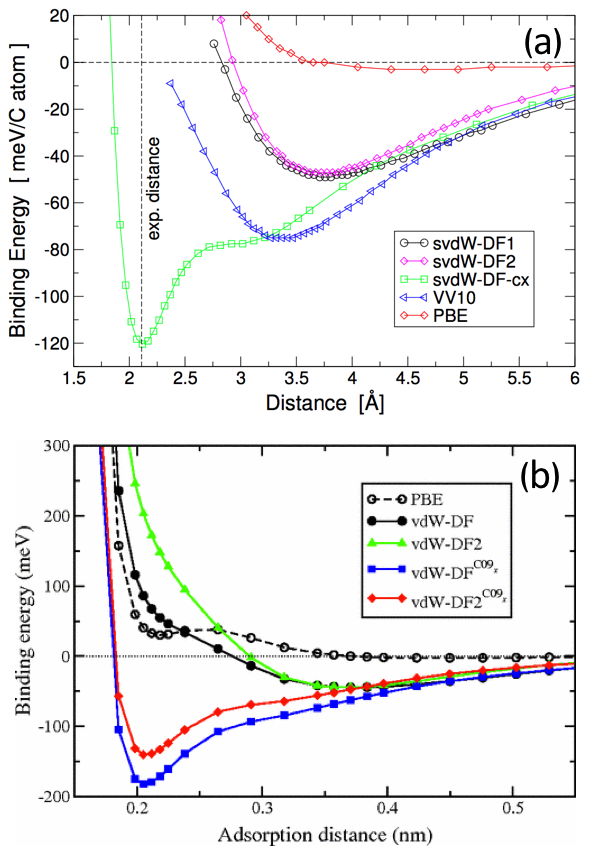
\includegraphics[scale=1.0,keepaspectratio]{Figs/svdW.png}
    \caption{(a) Taken from supplementary material given by~\cite{Thonhauser2015PRL} depicting the equilibrium distances and binding energies for graphene on the Ni 111 surface. Examined with different spin polarised vdW functionals and comparing it with other non-local functionals. The experimental value for equilibrium binding distance is taken from~\cite{Gamo1997}. (b) Taken from~\cite{Hamada2010} showing the same curve as in (a) but emphasising Cooper's version of functional~\cite{Cooper2010}, these calculations are spin-polarised as well}
    \label{fig:svdW}
\end{figure}
\begin{figure}
    \centering
    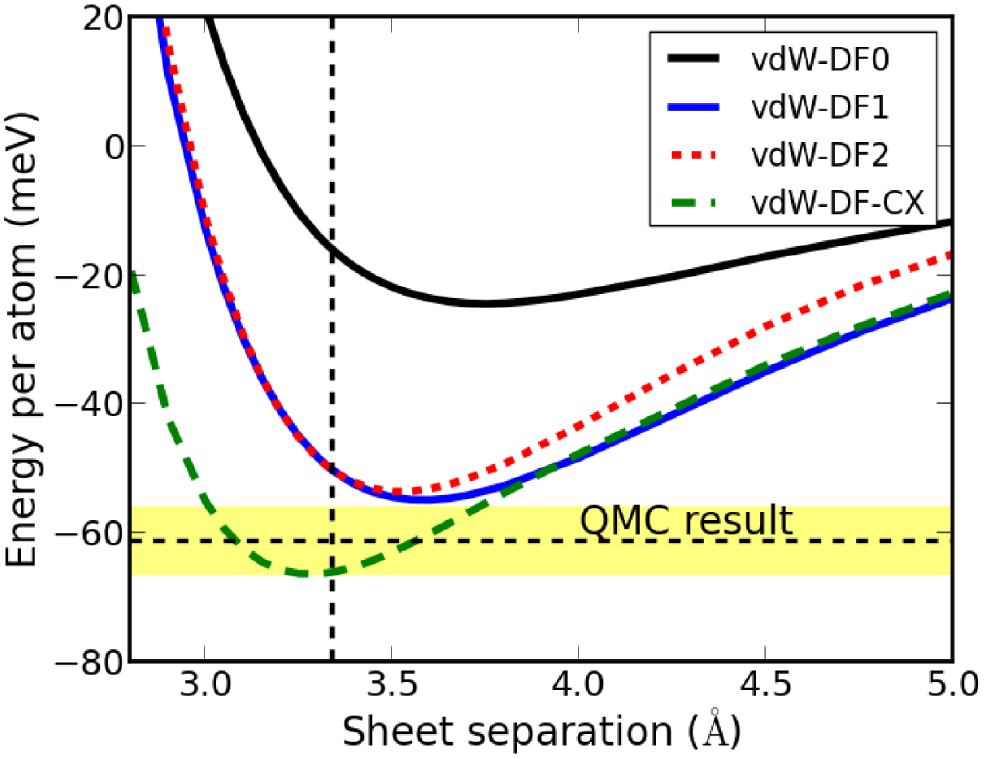
\includegraphics[scale=1.0,keepaspectratio]{Figs/svdWGraphite.jpg}
    \caption{Taken from~\cite{vdWreview} benchmarking the performance of the vdW-DF-cx functional versus the earlier versions of vdW-DFs, the experimental value represented in the vertical dashed line and the quantum Monte Carlo and RPA result (from~\cite{Lebegue2010PRL, Spanu2009PRL}) with the horizontal dashed line with yellow error bar regions. The figure is a result of a calculation of the inter-layer separation values within graphite.}
    \label{fig:svdWGraphite}
\end{figure}

As the non-local correlation term contains a double spatial integral as shown in equation (\ref{vdWeqn2}) resulting in six-dimensional integrals, it gets quite computationally expensive calculating it the way it was introduced either none-self-consistently~\cite{Dion2004} or self-consistently~\cite{thonhauser2007van} making it an $\mathcal{O}(n^2)$ problem. Román-Pérez together with José M. Soler\cite{NlogNalgorithm} calculated the integral self-consistently by factorising the integration kernel and use the fast Fourier transforms to evaluate the self-consistent potential, total energy, and atomic forces resulting in a reduced computational complexity of $\mathcal{O}(n\log{}n)$ operations. Regarding calculational time, this method is $\approx 10^3$ times less expensive than the original implementation and $\approx 10$ times costly when compared to the PBE cost. This algorithm is widely implemented in the different DFT codes nowadays. Sabatini et al.~\cite{Sabatini2013} had also introduced algorithm efficiently implementing the VV10 functionals, introducing the rVV10 functional.

As a quick overview on the efficiency of the proposed non-local functionals and benchmarking their results with experimental results: Björkman et al.~\cite{Bjorkman2012areWeReady} calculated the energy per unit area of the surface of the hexagonal hafnium ditelluride (HfTe$_{\textrm 2}$) TMDC for a wide range of different c lattice constant values. They got minima at the experimental value via the VV10 functional~\cite{Oleg2010} as well as a close performance achieved by the DFT-D correction~\cite{Grimme2006} as depicted in Fig. \ref{fig:vdWcomparison}a. HfTe$_{\textrm 2}$ is a layered semi-metal as graphene where its layers are intact together via vdW interactions. Similarly, Berland et al.~\cite{Berland2014vdWxc} benchmarked the vdW-DF-cx with the experimental as well as the accurate RPA results for graphite lattice constants revealing excellent agreement as shown in Fig. \ref{fig:vdWcomparison}b. 
\begin{figure}
    \centering
    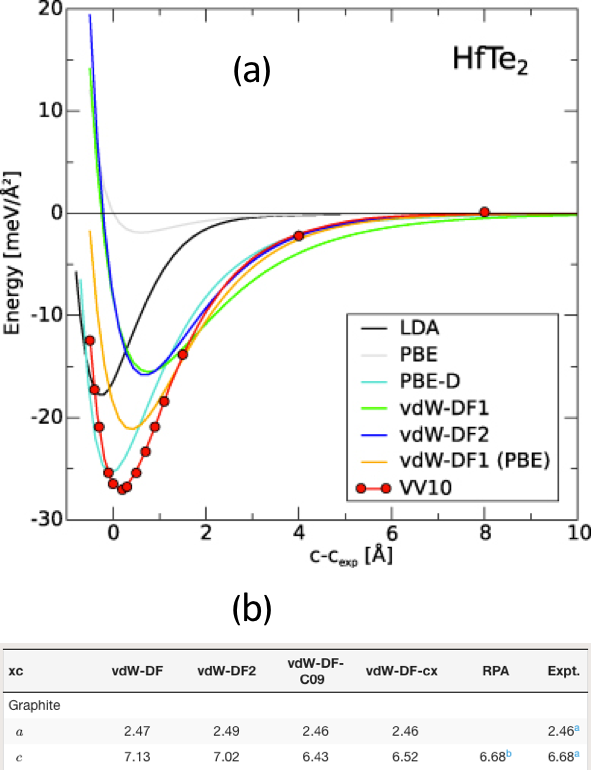
\includegraphics[scale=1.0,keepaspectratio]{Figs/vdWcomparison.png}
    \caption{(a) excerpt from~\cite{Bjorkman2012areWeReady} showing the performance of various dispersion functionals dealing with the dispersion forces governed by vdW showing both the densities overlaop pauli repulsion compression side as well the vdW attraction slope. (b) taken from~\cite{Berland2014vdWxc} showing results from differnet vdW functionals on graphite lattice constants.}
    \label{fig:vdWcomparison}
\end{figure}
In conclusion, The vdW functionals have been proven to be a not very expensive regarding computational time except for some complicated accurate versions, complicating the kernel. They give a promising solution for high accuracy calculations achieving the so-called "chemical" accuracy. That, in turn, can help \textit{ab-initio} scientists who are always concerned about solving the optimisation problem of accuracy versus calculation cost. Of course, with further development in computing technologies, scientists can shift their interest towards the exact method of quantum Monte Carlo (QMC) or random phase approximation (RPA). The open question is whether it is crucial to the specific problem under study or not. Worth mentioning, comparing DFT results with QMC or RPA is advantageous where we can avoid experimental uncertainties and contributions from the thermal motion that are not dealt in BO approximation.
\subsection{vdW and 2D materials}
As discussed in previous paragraphs, vdW functionals had a long run of success if we benchmark it with accurate methods in quantum Monte Carlo and PRA. In 2D materials, the uses of vdW functionals are materialised in describing the physisorption of molecules towards 2D surfaces, including graphene, TMDC and other valleytronics materials. That has been studied extensively in literature~\cite{Berland2013, Moses2009, Kleis2008, Berland2011,Joel2012, Bergvall2011, Svetla2010, Duy2012, Lee2011H2Cu111, Elias2012, Jiang2009, COOPER201234, Bjork2010, Martin2011}.
\section{Planewaves and pseudopotentials}
\label{planewaves}
In the thesis' related manuscripts, we used planewaves together with pseudopotentials, where planewaves is a type of basis set. With the help of a basis set, an arbitrary function (for example a charge density of a wave function) can be written as a sum of the basis functions weighted with coefficients. 

Equation~\ref{PWeigenfunc} expands the eigenstates in terms of an infinite number of plane waves with corresponding coefficients. $c_{\vec{K}}^{n,\vec{k}}$.
\begin{equation}
\psi_{\vec{k}}^{n}(\vec{r}) \, = \, \sum_{\vec{K}}c_{\vec{K}}^{n,\vec{k}}e^{(\vec{k}+\vec{K}).\vec{r}}
\label{PWeigenfunc}
\end{equation}

It is impossible to numerically evaluate an infinite number of coefficients for the basis set. Therefore the solution is limited to $\vec{K}$ by specifying a limiting value $\vec{K}_{\text{max}}$, which is the radius of a sphere in the reciprocal space whose centre is the origin. Thus, the limiting factor for all the $\vec{K}$ is set to $\vec{K} \leq \vec{K}_{\text{max}}$. The corresponding free electron energy is called the \textit{cut-off energy} which is expressed in equation~\ref{cutoffE} as:
\begin{equation}
E_{\text{cut-off}} \, = \, {{\hbar^2 K_{\text{max}}^2}\over{2m_e}}
\label{cutoffE}
\end{equation}
Here, $m_e$ is the electron mass.
\subsection{Pseudopotentials and vdW functionals}
As the electronic wave functions are very steep in the close neighbourhood of the nucleus and the limitation introduced by choosing a plane wave cutoff will cause high inaccuracy. Replacing the potential in the close vicinity of the nucleus with a pseudopotential that models the electronic wave functions properly in the interstitial region can be a good solution to the inaccuracy issue. Since most of the chemical bonding appears away from the nucleus in the inter-atomic region, the result of using pseudopotentials has a much lower computational cost for the same accuracy.

Ikutaro et al.~\cite{Ikutaro2011} have done a fascinating study comparing vdW electronic structure calculations performed using pseudopotentials generated with PBE functional versus pseudopotentials generated with consistent vdW functionals, they found out that the binding distances are slightly underestimated with pseudopotentials generated with PBE functional, while the binding energies are slightly overestimated. Meanwhile, the electronic structure regarding band structures is not altered. These differences are still in the range of the chemical accuracy with an error of 36 meV. Thus, it is safe and considerably still accurate to use pseudopotentials generated by PBE within vdW electronic structure calculation. It is a common practice to use PBE pseudopotentials as the vdW-DF non-local functionals utilise their exchange term.
\section{Summary}
In summary, we have enlightened the basis of DFT and how dispersion interactions are treated within. Dispersion interactions are essential to be considered when dealing with layered materials and describing adsorption properties. As there are several ways to describe it, thus, we choose the one suitable for the specific system under study.
\endinput